\subsection{I postulati di Einstein}\label{Sec:postulati}
Per giungere ad una formulazione coerente della dinamica dei corpi carichi Einstein, nel suo articolo del 1905$^{\cite{Einstein1905}}$, propose di modificare gli assunti alla base della meccanica classica per prediligere un modello coerente con l'elettromagnetismo di Maxwell.\\Infatti all'epoca erano noti alcuni risultati sperimentali che giocavano a sfavore della concezione classica della meccanica, primo fra tutti l'esperimento di Michelson e Morley che avrebbe dovuto consentire di misurare la velocità della Terra rispetto all'etere luminifero, detta vento d'etere. L'esperimento ebbe un esito inaspettato, infatti non fu possibile misurare alcun vento d'etere portando i fisici a tre possibili spiegazioni: o l'Etere si muove assieme alla Terra, o l'apparato sperimentale si contrae lungo la direzione del moto terrestre oppure non esiste alcun Etere e la luce si propaga alla medesima velocità in ogni direzione e per ogni osservatore.\\
\newpage
Einstein pose quindi a fondamento della sua teoria due postulati:
\begin{itemize}
    \item Il principio di relatività: basato sull'assunzione che esistano  una serie di sistemi di riferimento detti inerziali, reciprocamente in moto rettilineo uniforme, in cui le leggi della fisica sono identicamente valide.
    \item Il principio di costanza della velocità della luce: il quale asserisce che la luce nello spazio vuoto si propaghi sempre con modulo della velocità determinato ed identico per ogni osservatore inerziale, che si indicherà con $c$. 
\end{itemize}
Il primo si è lo stesso principio della meccanica classica mentre il secondo è una diretta conseguenza dell'esperimento di Michelson e Morley il cui risultato viene spiegato senza la necessità dell'introduzione dell'etere e di un sistema di riferimento privilegiato. Inoltre si continua ad intendere spazio e tempo come due enti omogenei e isotropi.\\

La primissima conseguenza dell'assunzione di questi due postulati è la non validità delle trasformazioni di Galileo. Infatti secondo queste un moto di velocità $\vec{v}$ in un sistema $K$, se osservato in un sistema $K'$, nel quale $K$ si muove a velocità $\vec{V}$, risulterà in un moto a velocità $\vec{v}+\vec{V}$. Il secondo postulato però richiede che se tale moto è di un fascio di luce questo debba risultare sia in $K$ che in $K'$ in un moto con modulo della velocità pari a $c$, in totale disaccordo con le trasformazioni di Galileo.\\

Inoltre nel suo articolo Einstein stesso propose, dopo aver enunciato i postulati, un esperimento mentale che consente di mostrare come questi siano in diretto conflitto con le assunzioni classiche dell'assolutezza del tempo e delle lunghezze. Si considerino due orologi reciprocamente a riposo posizionati in due punti detti $A$ e $B$. Einstein osservò che ogni orologio è in grado di misurare intervalli temporali solamente per eventi che avvengono nello stesso punto in cui ognuno è posizionato, questo poiché diventa necessario tener conto della velocità finita della luce che quindi non propagandosi istantaneamente genera dei ritardi nella percezione degli eventi lontani.\\ Il secondo postulato consente però di sincronizzare gli orologi così che sia possibile confrontare i tempi misurati in $A$ e in $B$. In primo luogo si ipotizzi di far partire all'istante $t_A=0$, misurato dal primo orologio, un fascio di luce che viaggia da $A$ e giunge in $B$ quando l'orologio posizionato in tale punto segna un tempo $t_B$. In $B$ il fascio è riflesso e fa ritorno in $A$ quando il relativo orologio segna un tempo $t_A$. Poiché per il principio di costanza della velocità della luce il fascio luminoso deve propagarsi in ogni direzione con la stessa velocità e la distanza tra i due orologi è fissata e costante allora il tempo impiegato dalla luce per andare da $A$ a $B$ e vice versa deve essere il medesimo. Si conclude quindi che i due orologi sono sincronizzati solamente se vale:
\begin{equation}
    2t_B=t_A.
    \label{SinconizazioneOrologi}
\end{equation}
Chiaramente se l'orologio nel punto $A$ si è rivelato sincrono con quello nel punto $B$, tramite la procedura appena descritta, è chiaro che è altrettanto vero che quello posto in $B$ è sincrono con quello posto in $A$ e che se si considera un orologio posto in un terzo punto $C$ che risulta sincrono con quello posto in $B$ allora questo terzo orologio è sincrono con quello nel punto $A$.\\Così facendo è possibile assegnare un immaginario orologio ad ogni punto dello spazio in maniera tale che siano tutti sincroni tra loro e sia possibile determinare quando due eventi lontani fra loro avvengono nello stesso istante in un determinato sistema di riferimento inerziale.\\
Fatta propria questa osservazione è possibile procedere analizzando l'esperimento mentale.
\begin{figure}[H]
    \centering
    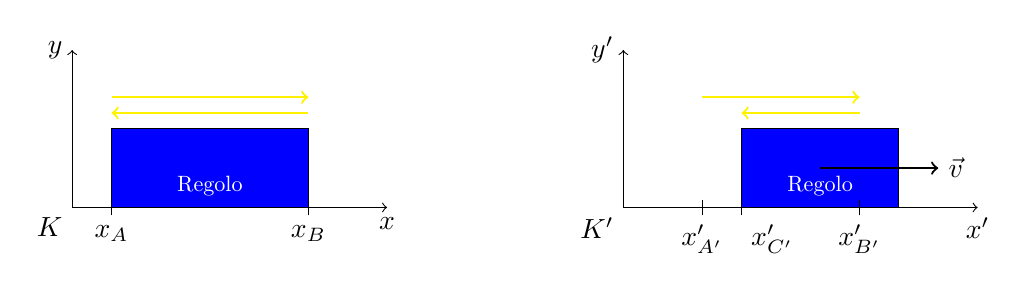
\begin{tikzpicture}
        \draw[->,black] (0,0)node [anchor=north east]{$K$} -- (4,0) node[anchor=north ]{$x$};
        \draw[->,black] (0,0) -- (0,2) node[anchor= east]{$y$};
        \draw[fill=blue] (0.5,0) rectangle node[anchor=north,scale=0.8,white]{Regolo} (3,1);
        \draw[black] (0.5,-0.1) node[anchor=north]{$x_A$} -- (0.5,0.1);
        \draw[black] (3,-0.1) node[anchor=north]{$x_B$} -- (3,0.1);
        \draw[yellow,->,thick] (0.5,1.4) -- (3,1.4);
        \draw[yellow,<-,thick] (0.5,1.2) -- (3,1.2);

        \draw[->,black] (0+7,0)node [anchor=north east]{$K'$} -- (4.5+7,0) node[anchor=north ]{$x'$};
        \draw[->,black] (0+7,0) -- (0+7,2) node[anchor= east]{$y'$};
        \draw[fill=blue] (1.5+7,0) rectangle node[anchor=north,scale=0.8,white]{Regolo} (3.5+7,1);
        \draw[black] (1+7,-0.1) node[anchor=north]{$x_{A'}'$} -- (1+7,0.1);
        \draw[black] (1.5+7,-0.1) node[anchor=north west]{$x_{C'}'$} -- (1.5+7,0.1);
        \draw[black] (3+7,-0.1) node[anchor=north]{$x_{B'}'$} -- (3+7,0.1);
        \draw[yellow,->,thick] (1+7,1.4) -- (3+7,1.4);
        \draw[yellow,<-,thick] (1.5+7,1.2) -- (3+7,1.2);
        \draw[black,->,thick] (2.5+7,.5) -- (4+7,.5) node[anchor=west]{$\vec{v}$};
    \end{tikzpicture}
    \caption{Rappresentazione dell'esperimento mentale di Einstein.}
    \label{fig:esperMentale}
\end{figure}
Si consideri un regolo di lunghezza $l$ in un sistema di riferimento ad esso solidale detto $K$. Si considerino anche due orologi sincroni posti nelle due estremità del regolo dette $A$ e $B$, se si ripete quanto appena fatto per la sincronizzazione degli orologi si deve osservare che il tempo impiegato dalla luce per muoversi da un estremo ad un altro è il medesimo in entrambe le direzioni.\\ In un sistema $K'$ si osserva il regolo in moto a velocità $v$ lungo la direzione in cui la parte lunga del regolo poggia. Sia detto $A'$ il punto del sistema $K'$ in cui si osserva l'emissione del fascio di luce dalla prima estremità del regolo, $B'$ il punto, sempre in $K'$, in cui si osserva la riflessione del fascio nel secondo estremo del regolo ed infine $C'$ il punto in $K'$ in cui si osserva il fascio fare ritorno alla prima estremità. In ognuno dei tre punti è presente un orologio sincronizzato con gli altri del sistema $K'$ in maniera da osservare l'emissione del fascio ad un tempo $t'_{A'}=0$. Se $t'_{B'}$ è l'istante in cui si osserva la riflessione in $B'$, $t'_{C'}$ è l'istante in cui il fascio fa ritorno al primo estremo del regolo e $l'$ è la lunghezza del regolo misurata nel sistema $K'$ allora è possibile determinare in funzione di questi tempi le distanze tra i punti $A',\ B'$ e $C'$, infatti queste dipenderanno in parte dalla distanza percorsa del regolo e in parte dalla sua lunghezza:
\begin{flalign*}
    &\Delta x'_{A'B'}=x'_{B'}-x'_{A'}=v(t'_{B'}-t'_{A'})+l'=vt'_{B'}+l',\\
    &\Delta x'_{B'C'}=x'_{B'}-x'_{C'}=l'-v(t'_{C'}-t'_{B'}).
\end{flalign*}
Queste due distanze sono quelle percorse dal fascio luminoso rispettivamente in tempi $t'_{B'}$ e $t'_{C'}-t'_{B'}$, per cui si ottiene:
\begin{flalign*}
    \Delta x'_{A'B'}=ct'_{B'}=vt'_{B'}+l' \quad &\Rightarrow\qquad t'_{B'}=\frac{l'}{c-v},\\
    \Delta x'_{B'C'}=c(t'_{C'}-t'_{B'})=l'-v(t'_{C'}-t'_{B'}) \qquad &\Rightarrow\quad t'_{C'}-t'_{B'}=\frac{l'}{c+v}.
\end{flalign*}

Questa semplice osservazione consente di concludere che i postulati enunciati da Einstein non ammettono la possibilità di assumere tempi assoluti: infatti l'osservatore in $K'$ osserva che il fascio di luce impiega più tempo per giungere al secondo estremo di quanto ne trascorra tra la riflessione e il suo ritorno al primo estremo, mentre invece l'osservatore in $K$, solidale con il regolo, osserva tempi identici per questi due tragitti. Una volta sviluppata matematicamente questa nuova teoria della relatività si osserverà che in maniera analoga pure le lunghezze non possono più essere considerate assolute.